%------------------------
% Shared preamble for cv.tex and cover_letter.tex
% Based on: Resume Template by Anubhav Singh (https://github.com/xprilion), MIT
%
% This file is language-independent and must stay IDENTICAL on every branch.
% Language-specific text (labels, dates, contact details) lives in refs/.
%------------------------

\usepackage{latexsym}
\usepackage[empty]{fullpage}
\usepackage{titlesec}
\usepackage{marvosym}
\usepackage[usenames,dvipsnames]{color}
\usepackage{verbatim}
\usepackage{enumitem}
\usepackage[hidelinks]{hyperref}
\usepackage{fancyhdr}
\usepackage{tabularx}
\usepackage{graphicx}

\newlength{\origtextwidth}

\pagestyle{fancy}
\fancyhf{}
\fancyfoot{}
\renewcommand{\headrulewidth}{0pt}
\renewcommand{\footrulewidth}{0pt}

% Horizontal margins (vertical ones are set per document)
\addtolength{\oddsidemargin}{-0.530in}
\addtolength{\evensidemargin}{-0.375in}
\addtolength{\textwidth}{1in}
\setlength{\footskip}{3.60004pt}

\urlstyle{rm}
\raggedbottom
\raggedright
\setlength{\tabcolsep}{0in}

%-----------SECTION FORMAT-----------------
\titleformat{\section}{
  \vspace{-2pt}\scshape\raggedright\large\bfseries
}{}{0em}{}[\color{black}\titlerule \vspace{-4pt}]

%-----------RESUME COMMANDS-----------------
\newcommand{\resumeItem}[2]{\item\small{\textbf{#1}{: #2}}}
\newcommand{\resumeItemPlain}[1]{\item\small{#1}}
\newcommand{\resumeSubheading}[4]{
  \vspace{-1pt}\item
    \begin{tabular*}{0.97\textwidth}{l@{\extracolsep{\fill}}r}
      \textbf{#1} & #2 \\
      \textit{#3} & \textit{#4} \\
    \end{tabular*}\vspace{-2pt}
}
\newcommand{\resumeSubItem}[2]{\resumeItem{#1}{#2}\vspace{-1pt}}
\renewcommand{\labelitemii}{$\circ$}
% Public evidence for a project: \repo{ItsShriks/ur5_simulation}
\newcommand{\repo}[1]{\href{https://github.com/#1}{\raisebox{-1pt}{
\includegraphics[height=8pt]{images/github.png}}\,\nolinkurl{github.com/#1}}}
\newcommand{\resumeSubHeadingListStart}{\begin{itemize}[leftmargin=*,itemsep=0.5pt,parsep=0pt,topsep=1pt]}
\newcommand{\resumeSubHeadingListEnd}{\end{itemize}}
\newcommand{\resumeItemListStart}{\begin{itemize}[itemsep=0.5pt,parsep=0pt,topsep=1pt]}
\newcommand{\resumeItemListEnd}{\end{itemize}\vspace{-2pt}}

%-----------REFS MECHANISM-----------------
% refs/*.tex hold the master content as named entries:
%     \defref{exp:navilan}{ ...LaTeX... }
% tex/*.tex pull an entry in unchanged with:
%     \useref{exp:navilan}
% or write a tailored version of it inline instead.
\newcommand{\defref}[2]{\expandafter\newcommand\csname cvref@#1\endcsname{#2}}
\newcommand{\useref}[1]{%
  \ifcsname cvref@#1\endcsname
    \csname cvref@#1\endcsname
  \else
    \errmessage{Unknown ref `#1' -- check refs/*.tex}%
  \fi}

%-----------CANDIDATE DATA (overridable)-----------------
\newif\ifcvphoto
\cvphototrue
\def\cvdob{}  % shown in the header only when non-empty

%===========================================================================
% refs/Personal_Info.tex  --  MASTER (English)
% Source of truth. Never tailor this file; tailor tex/ instead.
%===========================================================================

%-----------CONTACT-----------------
\newcommand{\cvname}{Shrikar Nakhye}
\newcommand{\cvlocation}{Bonn, Germany}
\newcommand{\cvemail}{nakhyeshrikar@icloud.com}
\newcommand{\cvphone}{+49 152 19520308}
\newcommand{\cvlinkedin}{https://www.linkedin.com/in/shrikar-nakhye-053262188/}
\newcommand{\cvgithub}{https://github.com/ItsShriks}
\newcommand{\cvscholar}{https://scholar.google.com/citations?user=-kVcoO8AAAAJ\&hl=en}
% Date of birth is not shown on English CVs (set \cvdob to show it)
% \renewcommand{\cvdob}{30 August 2000}

%-----------LANGUAGE STRINGS-----------------
\newcommand{\cvlabeladdress}{Address}
\newcommand{\cvlabelemail}{Email}
\newcommand{\cvlabeldob}{Date of Birth}
\newcommand{\cvcity}{Bonn}
\newcommand{\cvdate}{\today}
\newcommand{\cvclosing}{Kind regards,}

%-----------HEADLINES-----------------
\defref{headline}{Robotics Software Engineer | Autonomous Systems Engineer | Robot Navigation Engineer | Robotics Simulation Engineer | Robotics Integration Engineer}

%-----------SUMMARY-----------------
\defref{summary}{Robotics Engineer and Autonomous Systems professional with 4+ years of experience in robotics software development, robot perception, autonomous navigation, simulation, machine learning and system integration. Currently pursuing a Master of Science in Autonomous Systems in Germany with hands-on experience developing ROS and ROS 2-based applications for mobile robots, manipulators and autonomous platforms. Strong expertise in robot navigation, SLAM, sensor fusion, coordinate frame management, point cloud processing, computer vision and robotic simulation environments. Experienced in designing navigation stacks, perception frameworks, robot control systems and autonomous workflows using ROS 2, OpenCV, PyTorch, Open3D, Gazebo and Webots. Passionate about building scalable robotic solutions for industrial automation, autonomous mobility and next-generation intelligent systems.}

%-----------KEY FACTS (for tailoring; never invent beyond these)-----------------
% Metrics : 95% tracking success rate (b-it bots, Toyota HSR)
%           Completed the Help Me Carry task at RoboCup German Open 2025 (@Home, b-it bots)
%           15% segmentation accuracy improvement (H-BRS research)
%           90-95% accuracy, fully offline OCR/layout-detection ensemble on low-end CPUs (Navilan)
%           Scrum Master of a 10-member engineering team (Sakar Robotics)
% Languages: English C2, German B2, Hindi native, Marathi native
% Preferred locations: Munich | Stuttgart | Germany | Remote
% Work authorization: Germany

%===========================================================================
% refs/Work_Experience.tex  --  MASTER (English)
% Source of truth. Never tailor this file; tailor tex/Work_Experience.tex.
% Entry format: \resumeSubheading{Role}{Dates}{Organisation}{Location}
%===========================================================================

\defref{exp:navilan}{
    \resumeSubheading
      {Student Assistant}{Jul 2025 -- Apr 2026}
      {Navilan Solutions}{Bonn, Germany}
      \resumeItemListStart
        \resumeItemPlain{Developed high-performance \textbf{C++ and Qt}-based desktop applications and automated \textbf{Python} telemetry services for document validation and vision pipelines.}
        \resumeItemPlain{Built a \textbf{fully offline} document layout detector and OCR ensemble (DocTR, Tesseract, EasyOCR) with image preprocessing, reaching \textbf{90--95\% accuracy} on multilingual text and tables while running on \textbf{low-end CPUs}.}
        \resumeItemPlain{Dockerized deployment workflows and established automated test suites and CI/CD quality gates, ensuring reproducible system builds and reliable release management.}
        % No metrics for this bullet: release/usage figures are confidential.
      \resumeItemListEnd
}

\defref{exp:hbrs-ra}{
    \resumeSubheading
      {Research Assistant}{Oct 2024 -- Apr 2025}
      {Hochschule Bonn-Rhein-Sieg}{Bonn, Germany}
      \resumeItemListStart
        \resumeItemPlain{Developed CUDA-accelerated 3D point cloud segmentation algorithms for UAV datasets in \textbf{C++, Python (PyTorch) and Open3D} on embedded Linux/GPU hardware.}
        \resumeItemPlain{Achieved a \textbf{15\% accuracy improvement} through systematic sensor calibration, ground-truth label validation and model/pipeline optimization.}
        \resumeItemPlain{Conducted structured root-cause analysis on sensor timing jitter and measurement anomalies; maintained experiment tracking, evaluation frameworks and technical documentation for system bring-up.}
      \resumeItemListEnd
}

\defref{exp:sakar}{
    \resumeSubheading
      {Robotics Engineer, Technical Associate \& Centre Manager}{May 2021 -- May 2023}
      {Sakar Robotics / HunarPro Hub}{Pune, India}
      \resumeItemListStart
        \resumeItemPlain{Led a 10-member engineering team as Scrum Master, contributing to \textbf{7 autonomous robotic platforms} (\textbf{2 delivered end-to-end}); owned hardware commissioning and configuration management.}
        \resumeItemPlain{Configured coordinate frames, multi-sensor integrations (LiDAR, Encoders, IMU) and navigation architectures using \textbf{ROS / ROS 2}; built object detection workflows with \textbf{YOLO and TensorFlow}.}
        \resumeItemPlain{Designed robotic components in Fusion 360 / Inventor and converted CAD assemblies into optimized collision meshes and simulation-ready URDF assets.}
        \resumeItemPlain{Mentored robotics teams, supported automation laboratory development and contributed to IndiaSkills Mobile Robotics training programs.}
      \resumeItemListEnd
}

\defref{exp:learnbyresearch}{
    \resumeSubheading
      {Lead Researcher / Hardware Development Researcher}{May 2021 -- Dec 2021}
      {LearnByResearch}{Remote}
      \resumeItemListStart
        \resumeItemPlain{Designed and analyzed a 3-DOF robotic manipulator for object-picking applications; conducted kinematic analysis and simulation studies in SolidWorks and CATIA.}
        \resumeItemPlain{Developed a low-cost LiDAR scanner and configured SLAM workflows for indoor mapping applications; published findings in IEEE and international journals.}
      \resumeItemListEnd
}

\defref{exp:ssig}{
    \resumeSubheading
      {Robotics System Intern}{May 2019 -- Jul 2019}
      {SSIG Manufacturing Advancements Pvt. Ltd.}{Pune, India}
      \resumeItemListStart
        \resumeItemPlain{Programmed \textbf{ABB IRB1320 industrial robots} using \textbf{RAPID and RobotStudio}; designed automated motion sequences, pick-and-place tasks and monitored execution.}
        \resumeItemPlain{Calibrated Tool Center Points (TCP) and integrated industrial I/O and PLC monitoring streams; supported hands-on hardware troubleshooting and sensor verification.}
      \resumeItemListEnd
}

%-----------SIDE JOBS (for non-technical / retail roles only)-----------------
\defref{exp:retail-cashier}{
    \resumeSubheading
      {Cashier}{Oct 2023 -- Present}
      {REWE, Alnatura, Primark (mini-job and via Jobvalley / Zenjob)}{Bonn, Germany}
      \resumeItemListStart
        \resumeItemPlain{Handled \textbf{cashier duties} and ensured \textbf{accurate till reconciliation} in food and fashion retail.}
        \resumeItemPlain{Provided friendly, competent \textbf{customer service} at the checkout, including during peak hours.}
        \resumeItemPlain{Adapted quickly to different stores, POS systems and teams in \textbf{flexible assignments}.}
      \resumeItemListEnd
}

\defref{exp:edeka}{
    \resumeSubheading
      {Student Assistant -- Food Retail}{Aug 2025 -- Present}
      {EDEKA}{Bonn, Germany}
      \resumeItemListStart
        \resumeItemPlain{Stocked shelves and checked goods for \textbf{completeness, quality and best-before dates}.}
        \resumeItemPlain{Kept the sales floor and shelves \textbf{clean and organised}.}
        \resumeItemPlain{Advised customers and supported daily operations in \textbf{shift work}.}
      \resumeItemListEnd
}

%===========================================================================
% refs/Projects.tex  --  MASTER (English)
% Source of truth. Never tailor this file; tailor tex/Projects.tex.
% Entry format: \resumeSubheading{Title}{\repo{owner/name} or dates}{Tech stack}{Note}, then a bullet list
% Only link repositories that are public and contain the work described.
%===========================================================================

% Official team member, not employment -- list under Projects, never Experience.
\defref{proj:bitbots}{
    \resumeSubheading
      {b-it bots @Home -- RoboCup@Home Team}{Oct 2024 -- Present}
      {Perception \& Navigation Core Member $\cdot$ ROS 2, MediaPipe, OpenCV}{Extracurricular}
      \resumeItemListStart
        \resumeItemPlain{Developed a multimodal person-following and intention-awareness framework on the Toyota HSR robot using \textbf{ROS 2, MediaPipe and OpenCV}, achieving a \textbf{95\% tracking success rate}.}
        \resumeItemPlain{Engineered real-time pointing-gesture detection (ray intersection, \textbf{TF} transforms across camera, base and manipulator links), enabling the team to complete the \textbf{Help Me Carry} task at \textbf{RoboCup German Open 2025} (@Home).}
        \resumeItemPlain{Calibrated multi-sensor suites (RGB-D, LiDAR, odometry) and diagnosed hardware-software interface anomalies using \textbf{rosbag, RViz and Foxglove Studio}.}
        \resumeItemPlain{Integrated 3D object segmentation and spatial mapping using LiDAR and large-scale point cloud data; built visualization tools for robot reachability, frame alignment and camera visibility.}
        \resumeItemPlain{Engineered modular hardware adapters in \textbf{Modern C++ (C++17) and Python}; maintained reproducible containerized deployments via \textbf{Docker} and Git.}
      \resumeItemListEnd
}

\defref{proj:thesis}{
    \resumeSubheading
      {Continuous Mobile Manipulation Architecture}{\repo{ItsShriks/porta_ros2_ws}}
      {ROS 2, C++17, MPC, TSID, MuJoCo}{Master Thesis}
      \resumeItemListStart
        \resumeItemPlain{Designing a unified control and motion planning architecture coupling a visibility-aware MPC planner with a high-frequency TSID controller for continuous autonomous manipulation on mobile robot platforms.}
        \resumeItemPlain{Developing an asynchronous ROS 2 bridge and software adapters in \textbf{C++17} for trajectory interpolation, execution logic and real-time rigid-body dynamics validation.}
        \resumeItemPlain{Built a \textbf{MuJoCo} simulation of the MMO-700 mobile manipulator (MPO-700 base, UR5e arm, Robotiq 2F-85 gripper) with a full autonomous drive--reach--grasp--lift pipeline.}
      \resumeItemListEnd
}

\defref{proj:ur5}{
    \resumeSubheading
      {UR5 Robot Kinematics \& Motion Planning}{\repo{ItsShriks/ur5_simulation}}
      {ROS Noetic, KDL, MoveIt}{}
      \resumeItemListStart
        \resumeItemPlain{Developed a comprehensive kinematics simulation framework for a 6-DOF UR5 industrial robotic arm; implemented analytical inverse kinematics algorithms using \textbf{KDL}.}
        \resumeItemPlain{Designed and benchmarked collision-free trajectory generation and motion planning workflows using \textbf{MoveIt} and customized collision meshes.}
      \resumeItemListEnd
}

\defref{proj:amr-nav}{
    \resumeSubheading
      {Autonomous Mobile Robot Navigation Stack \& Commissioning}{}
      {ROS 2, Nav2, SLAM, EKF}{}
      \resumeItemListStart
        \resumeItemPlain{Integrated and validated an autonomous navigation stack using \textbf{ROS 2} and \textbf{Nav2} on a physical omnidirectional industrial platform; configured costmaps, path planners, recovery behaviors and multi-sensor localization (LiDAR, IMU, Encoders).}
        \resumeItemPlain{Designed and deployed a custom \textbf{Extended Kalman Filter (EKF)} node for sensor fusion and state estimation; supported frontier exploration.}
        \resumeItemPlain{Executed real-robot commissioning, map generation and trajectory validation; isolated edge-case anomalies using \textbf{rosbag, RViz and Docker logs}, documenting root causes in structured QA reports.}
      \resumeItemListEnd
}

\defref{proj:butler}{
    \resumeSubheading
      {Robot Butler \& Semantic Object Tagging}{\repo{ItsShriks/steve_hardware_bringup}}
      {ROS 2, Nav2, RTAB-Map, PyTorch, YOLO, LLM}{}
      \resumeItemListStart
        \resumeItemPlain{Engineered ROS 2 bring-up pipelines and hardware interfaces for a domestic service robot (\textbf{Neobotix MMO-700}: omnidirectional base, UR5e arm, Robotiq gripper, LiDARs, RealSense L515, IMU) with hands-off auto-start on boot.}
        \resumeItemPlain{Configured Nav2 and 3D SLAM (\textbf{RTAB-Map}) and integrated computer vision (\textbf{YOLO}, OpenYOLO3D, Mask3D) with LLM and vision-language models for semantic object retrieval and task planning.}
        \resumeItemPlain{Constructed automated sensor feeds, bounding-box annotations and evaluation scripts to validate multi-class detection and dynamic obstacle avoidance.}
      \resumeItemListEnd
}

\defref{proj:junglelook}{
    \resumeSubheading
      {JungleLook -- Label-free LiDAR Forest Point Cloud Segmentation}{\repo{ItsShriks/JungleLook}}
      {Python, PyTorch, PointNet++, Open3D}{}
      \resumeItemListStart
        \resumeItemPlain{Built a label-free segmentation pipeline for UAV point clouds: geometric features (DTM, height above ground, eigenvalues) generate pseudo-labels that train \textbf{PointNet / PointNet++}, reaching \textbf{0.80 validation mIoU} (preliminary, vs. pseudo-labels).}
        \resumeItemPlain{Registered field annotations to the LiDAR data with \textbf{RANSAC + ICP} at \textbf{98.8\% inliers} and \textbf{0.11\,m RMS}; packaged as a CI-tested library for CPU, CUDA and Apple MPS.}
      \resumeItemListEnd
    % Measured numbers (use only these):
    %   0.80 mIoU validation vs. pseudo-labels (ground 0.99, other 0.95, stump 0.46) -- always say "preliminary, vs. pseudo-labels"
    %   98.8% inliers / 0.11 m RMS annotation-to-LiDAR registration -- strongest hard number
    %   F1 0.31 rule-based stump detection vs. 129 annotated stumps -- only with "limited by data" context
    %   DO NOT USE: 11.8% / 93% from the broken v1 notebook; NO 15% was measured in this project
}

\defref{proj:prithvivision}{
    \resumeSubheading
      {PrithviVision -- Shadow-Casting Object Segmentation in Aerial Imagery}{\repo{ItsShriks/PrithviVision}}
      {U-Net, YOLO, Mask R-CNN}{}
      \resumeItemListStart
        \resumeItemPlain{Curated and annotated (YOLO format) an aerial-image dataset of Bonn and compared \textbf{U-Net, YOLO and Mask R-CNN} for detection and pixel-level segmentation of shadow-casting objects.}
      \resumeItemListEnd
}

\defref{proj:robocompanion}{
    \resumeSubheading
      {RoboCompanion -- Person-Following Assistive Robot}{\repo{ItsShriks/RoboCompanion}}
      {ROS, YOLOv8, RGB-D, Docker}{}
      \resumeItemListStart
        \resumeItemPlain{Built a modular, ROS-compatible person-tracking stack using \textbf{YOLOv8} and pose estimation with RGB-D (OpenNI2) cameras, packaged as a reproducible \textbf{Docker} deployment.}
      \resumeItemListEnd
}

\defref{proj:robograsp}{
    \resumeSubheading
      {RoboGrasp -- Object Recognition for Adaptive Grasping}{\repo{ItsShriks/RoboGrasp}}
      {Python, RGB-D, Point Clouds, EM}{}
      \resumeItemListStart
        \resumeItemPlain{Classified objects from RGB-D images and 3D point clouds with \textbf{Mixture-of-Gaussians} models trained via Expectation-Maximization to select grasp strategies.}
      \resumeItemListEnd
}

%===========================================================================
% refs/Education.tex  --  MASTER (English)
% Source of truth. Never tailor this file; tailor tex/Education.tex.
%===========================================================================

\defref{edu:msc}{
    \resumeSubheading
      {Hochschule Bonn-Rhein-Sieg}{Oct 2023 -- Feb 2027 (expected)}
      {Master of Science (M.Sc.) in Autonomous Systems}{Bonn, Germany}
      \resumeItemListStart
        \resumeItem{Thesis}{Coupling Visibility-Aware MPC with TSID for Continuous Mobile Manipulation.}
        \resumeItem{Activities}{Official Member of b-it bots @Home Team since October 2024; Honoured with DAAD Scholarship.}
      \resumeItemListEnd
}

\defref{edu:btech}{
    \resumeSubheading
      {Symbiosis Skills And Professional University}{Jul 2018 -- Jun 2022}
      {Bachelor of Technology (B.Tech.) in Mechatronics Engineering (CGPA: 8.787 / 10)}{Pune, India}
      \resumeItemListStart
        \resumeItem{Thesis}{Waste Separation System with a Robotic Manipulator.}
        \resumeItem{Activities}{Co-founder of Robo Club and Solar Club; Student Volunteer at Automotive Skills Development Council, India; Team Mentor for IndiaSkills Mobile Robotics Team.}
      \resumeItemListEnd
}

\defref{edu:hsc}{
    \resumeSubheading
      {Saket College}{Jun 2016 -- May 2018}
      {Higher Secondary Certification in Science (Grade: 60\%)}{Mumbai, India}
      \resumeItemListStart
        \resumeItem{Focus}{Mathematics, Physics and Chemistry.}
      \resumeItemListEnd
}

\defref{edu:ssc}{
    \resumeSubheading
      {Swami Vivekanand Vidyamandir}{Apr 2003 -- Apr 2016}
      {Secondary School Certification (Grade: 75.6\%)}{Mumbai, India}
      \resumeItemListStart
        \resumeItem{Activities}{Awarded as Best Student Representative; Co-Founder and President of Technology Club; Awarded as Best Science Club Vice President; Active in District Level Chess Tournaments.}
      \resumeItemListEnd
}

%===========================================================================
% refs/Skills.tex  --  MASTER (Deutsch)
% Alle Kenntnisse, die Shrikar tatsächlich hat. tex/Skills.tex wählt, ordnet
% und gruppiert daraus -- nie etwas in tex/ aufnehmen, das hier fehlt.
%===========================================================================

\defref{skill:robotics}{\resumeSubItem{Robotik \& Autonome Systeme}{ROS / ROS 2, Nav2, SLAM (RTAB-Map), EKF-Lokalisierung, Bewegungs- \& Pfadplanung, MoveIt, KDL, MPC, TSID, Mobile Manipulation, Koordinatentransformationen (TF), Kalibrierung \& Inbetriebnahme}}

\defref{skill:industrial}{\resumeSubItem{Industrierobotik \& Automatisierung}{ABB RAPID, RobotStudio, UR5 / UR5e, Robotiq-Greifer, Pick-and-Place, TCP-Kalibrierung, SPS- \& Industrie-I/O-Überwachung}}

\defref{skill:perception}{\resumeSubItem{Computer Vision \& Wahrnehmung}{Objekterkennung (YOLO), Semantische Segmentierung (2D / 3D), OCR (DocTR, Tesseract, EasyOCR), OpenCV, MediaPipe, Punktwolkenverarbeitung (Open3D), Multisensor-Fusion (LiDAR, RGB-D, IMU, Encoder, Radar, GPS)}}

\defref{skill:ml}{\resumeSubItem{Machine Learning}{PyTorch, TensorFlow, CUDA, PointNet / PointNet++, Behavioural Cloning, Modelltraining \& -evaluation, Datensatzerstellung \& Annotation, LLM- / VLM-Integration}}

\defref{skill:simulation}{\resumeSubItem{Simulation}{Gazebo, Webots, Isaac Sim, MuJoCo, URDF / Xacro, PX4, ArduPilot}}

\defref{skill:software}{\resumeSubItem{Software \& Tools}{Python, Modern C++ (C++17), C\#, Qt, CUDA, Linux, Git, Docker, CI/CD, FastAPI, NumPy, Pandas, JSON / YAML, rosbag, RViz, Foxglove Studio}}

\defref{skill:hardware}{\resumeSubItem{Hardware \& CAD}{Embedded Systems, NVIDIA Jetson, Arduino, Raspberry Pi, Fusion 360, Inventor, SolidWorks, CATIA, MATLAB, Simulink}}

\defref{skill:pm}{\resumeSubItem{Projektmanagement \& Zusammenarbeit}{Scrum / Agile (Scrum Master, 10-köpfiges Team), Prototypenvalidierung \& Tests, Ursachenanalyse, Technische Dokumentation \& QA-Berichte, Interdisziplinäre \& internationale Teamarbeit}}

\defref{skill:languages}{\resumeSubItem{Sprachen}{Deutsch (B2 -- fließend in Wort und Schrift), Englisch (C2 -- verhandlungssicher), Hindi \& Marathi (Muttersprachen)}}

%===========================================================================
% refs/Training_And_Certifications.tex  --  MASTER (English)
%===========================================================================

\defref{cert:ml}{\resumeSubItem{Machine Learning}{Completed comprehensive online specialization (final score: 91\%)}}
\defref{cert:cpp}{\resumeSubItem{C++}{Advanced C++ Programming \& Optimization for Robotic Systems; Introduction to C++}}
\defref{cert:python}{\resumeSubItem{Python}{Python for Robotics Applications; Python Intermediate; Introduction to Python}}
\defref{cert:matlab}{\resumeSubItem{MATLAB}{MATLAB Certified; Advanced MATLAB Training in GUI development, data extraction, and signal processing pipelines.}}

%-----------VOLUNTEERING (alternative section for non-technical roles)-----------------
\defref{vol:asdc}{\resumeSubItem{Automotive Skills Development Council, India}{Student Volunteer}}
\defref{vol:worldskills}{\resumeSubItem{WorldSkills India 2021}{Workshop Manager -- organised and prepared competition tasks}}
\defref{vol:school}{\resumeSubItem{School}{Awarded as Best Student Representative}}

%===========================================================================
% refs/Publications.tex  --  MASTER (English)
%===========================================================================

\defref{pub:strawberry}{\resumeSubItem{``Design and Analysis of Strawberry-Picking Industrial Robotic Arm''}{Published in \textit{IEEE -- Institute of Electrical and Electronics Engineers} (December 2022)}}

\defref{pub:3dprint}{\resumeSubItem{``Techniques in Improving Quality and Speed of 3D Printing''}{Published in \textit{IJRTI -- International Journal for Research Trends and Innovation} (April 2023)}}

\defref{pub:waste}{\resumeSubItem{``Waste Management Robotic Arm using MATLAB and Raspberry Pi''}{Published in \textit{NCETIR -- National Conference on Emerging Technologies in Interdisciplinary Research} (June 2022)}}

\defref{pub:lidar}{\resumeSubItem{``Development of Low-Cost LiDAR Scanner for Indoor Mapping''}{Published in \textit{IJISET -- International Journal of Innovative Science, Engineering \& Technology} (December 2021)}}

%===========================================================================
% refs/Interests.tex  --  MASTER (English)
%===========================================================================

\defref{int:general}{\resumeSubItem{Personal \& Technical Interests}{Continuous Learning, Traveling \& Exploring, Driving, Emerging Technologies, Chess, Robotics Prototyping}}

\defref{int:ai-safety}{\resumeSubItem{Technical \& Personal Interests}{Safety \& Robustness of AI Systems, Autonomous Systems, Open-Source Robotics, Chess, Traveling}}


%------------------------
% Shared page header (name, contact, photo). Must stay IDENTICAL on every branch.
% All text comes from macros defined in refs/Personal_Info.tex.
%------------------------
\definecolor{headerbg}{RGB}{242, 244, 247}

\newcommand{\cvheader}{%
  \setlength{\origtextwidth}{\textwidth}%
  \vspace*{-\dimexpr\topmargin+1in\relax}%
  \noindent
  \makebox[\origtextwidth][c]{%
    \colorbox{headerbg}{%
      \begin{minipage}{\paperwidth}
        \vspace*{25pt}
        \hspace{\dimexpr\oddsidemargin+1in\relax}%
        \begin{minipage}[c]{\ifcvphoto 0.72\fi\origtextwidth}
            \raggedright
            {\Huge \textbf{\cvname}} \\[6pt]
            \small
            \cvlabeladdress: \cvlocation \\
            \cvlabelemail: \href{mailto:\cvemail}{\cvemail} \\
            \ifx\cvdob\empty\else \cvlabeldob: \cvdob \\\fi
            \raisebox{-2pt}{
\includegraphics[height=10pt]{images/LinkedIn.png}}\ \href{\cvlinkedin}{LinkedIn} \quad
            \raisebox{-2pt}{
\includegraphics[height=10pt]{images/github.png}}\ \href{\cvgithub}{GitHub} \quad
            \raisebox{-2pt}{
\includegraphics[height=10pt]{images/Google_Scholar.png}}\ \href{\cvscholar}{Google Scholar}
        \end{minipage}%
        \ifcvphoto
        \hfill
        \begin{minipage}[c]{0.20\origtextwidth}
            \raggedleft
            {\setlength{\fboxsep}{0pt}\fbox{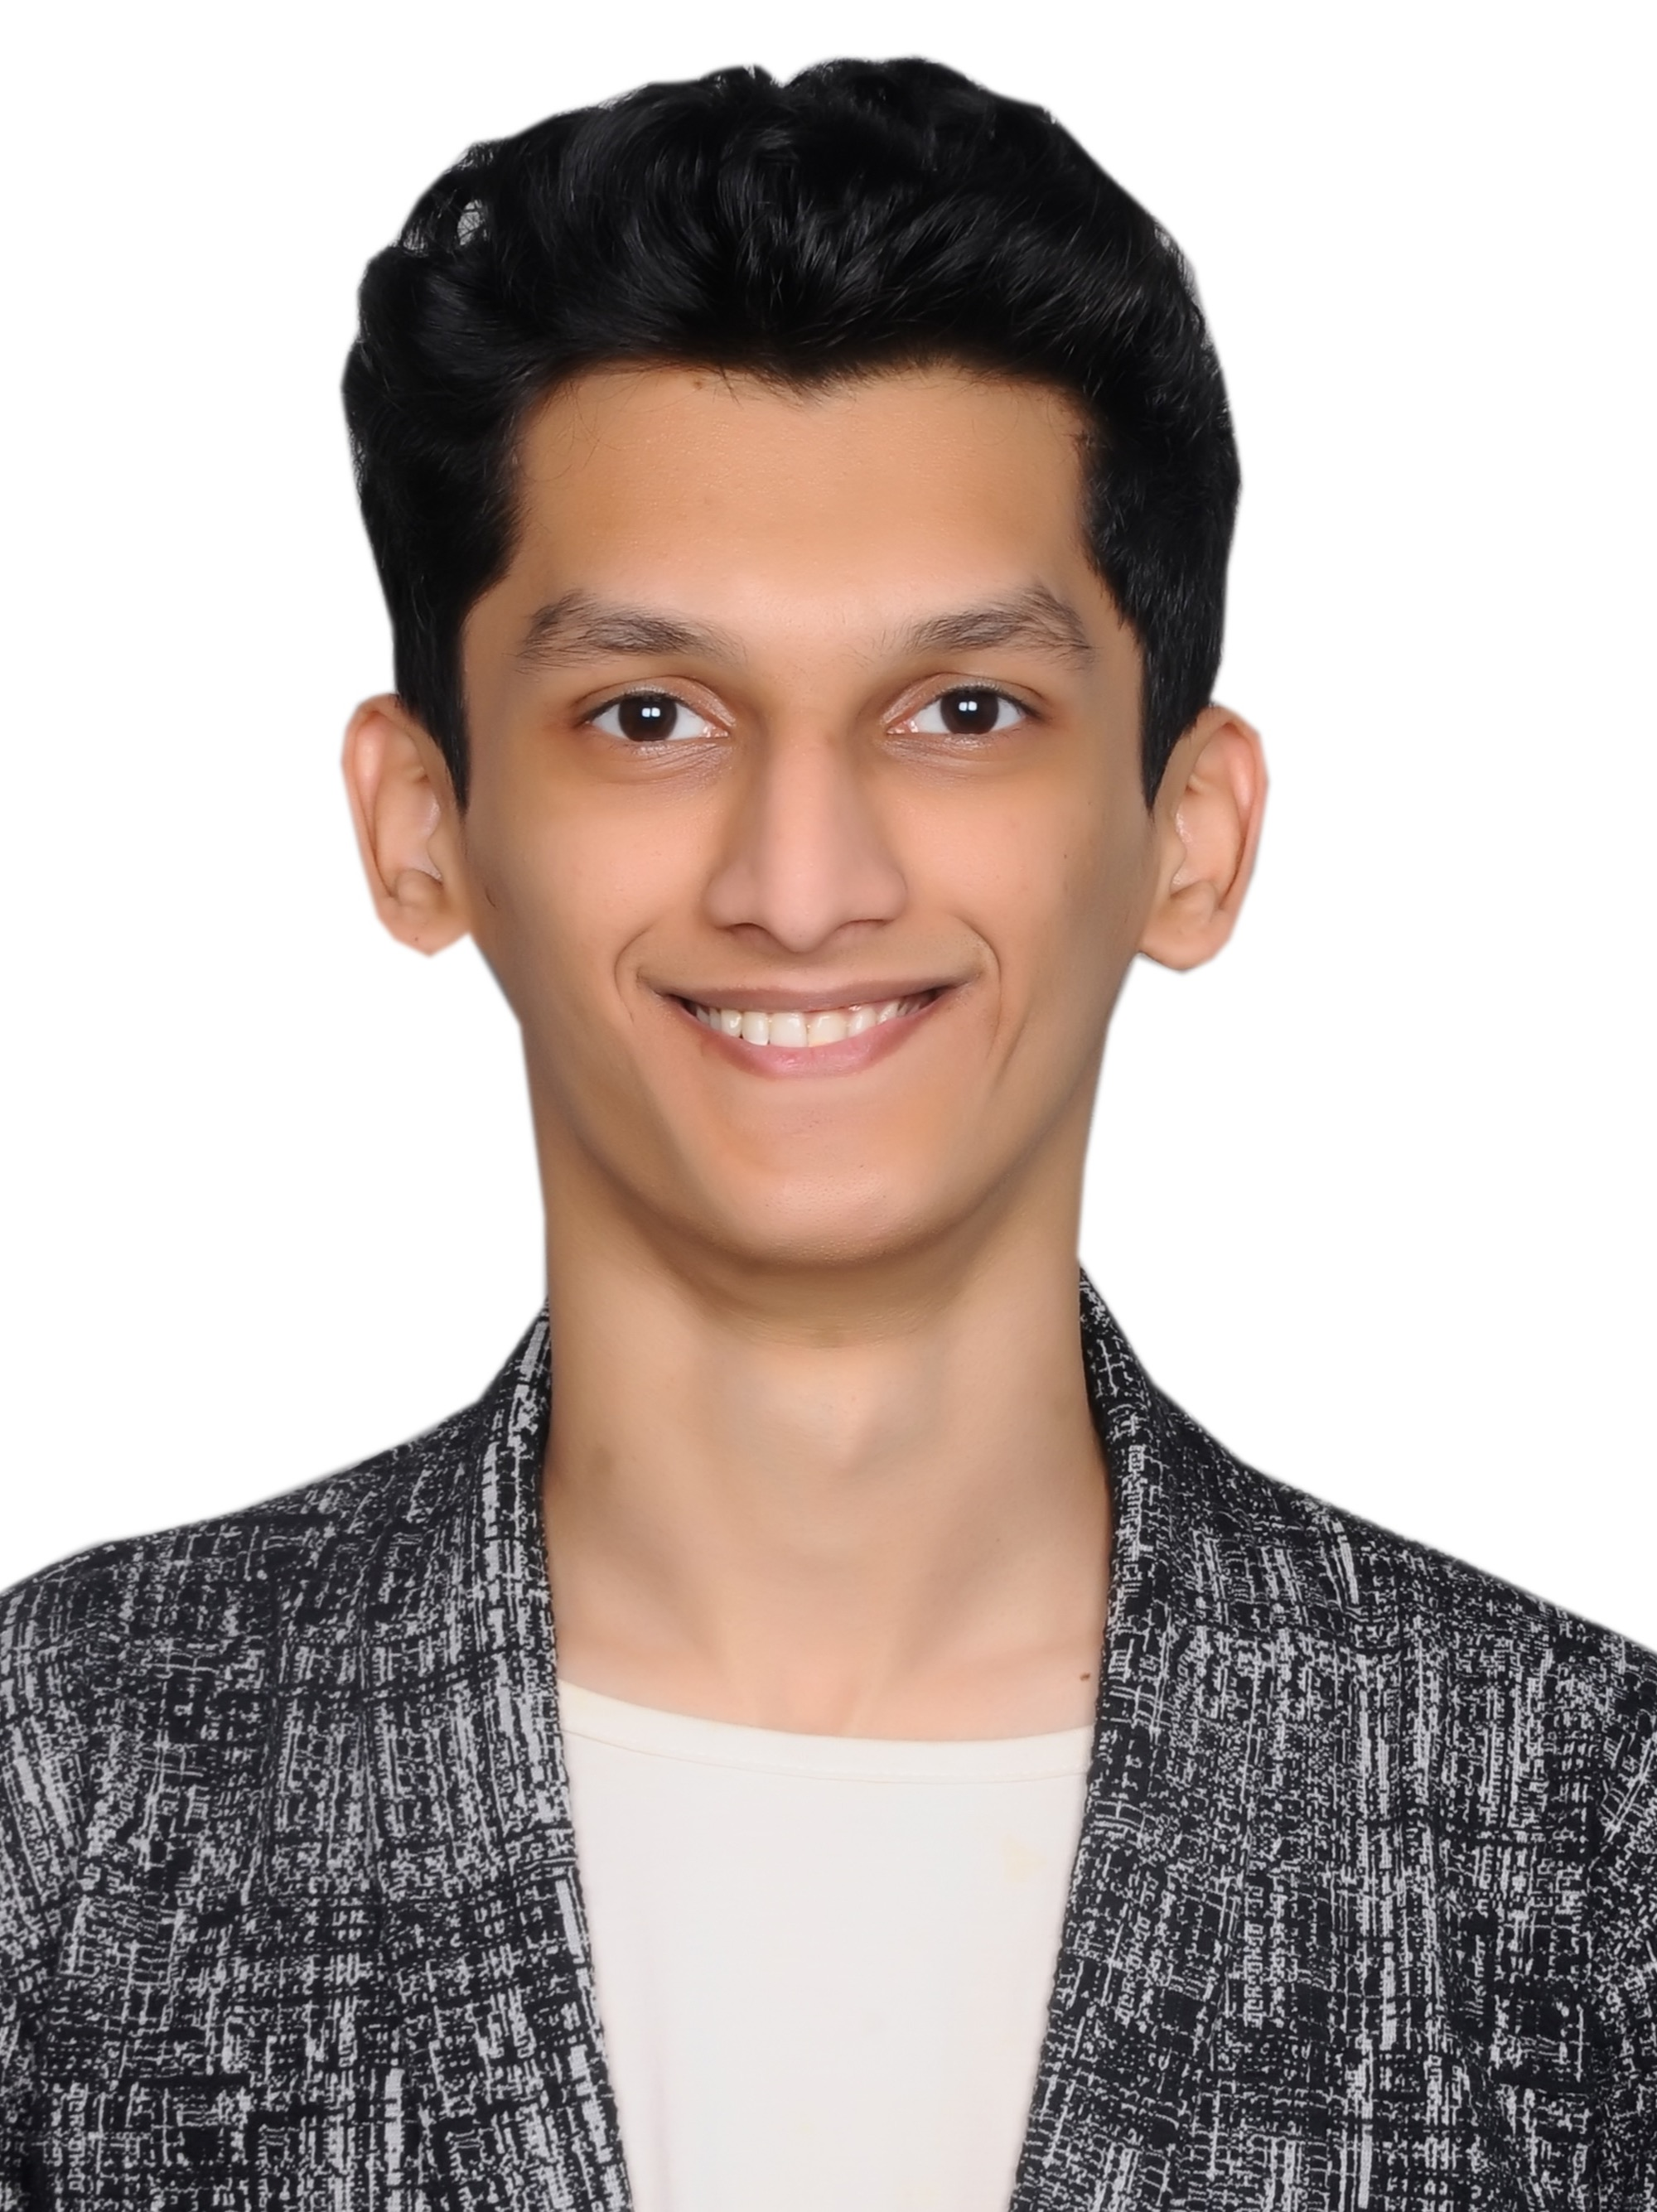
\includegraphics[width=2.5cm,height=3.3cm,keepaspectratio]{images/Self_Pic.jpg}}}
        \end{minipage}%
        \fi
        \hspace{\dimexpr\oddsidemargin+1in\relax}%
        \vspace{15pt}
      \end{minipage}%
    }%
  }%
}

